\section{Piecewise-quadratic Model}

The piecewise-quadratic model was covered extensively in \Cref{sec:setup.quad,sec:setup.quad.hyper}.
This section will cover choices of the varied parameters $\alpha$ and $\beta$ that are similar to the approach of \Cref{sec:setup.quad.hyper}.
Instead of defining the composite parameters as values of the model function, the parameters multiple parameters of the parameters $a_L, b_L, c_L, a_R, b_R,$ and $c_R$ are chosen to be influenced by the parameter $\alpha$.

Note that the definition of the piecewise-quadratic model is a little different in this section.
The domain is $[0, 6]$ and the borders are at $d_0 = 0, d_1 = \frac{3}{2}, d_2 = 3$, and $d_3 = \frac{9}{2}$.

\subsection{First Choice of Composite Parameters}

The parameters $a_R = 1 + \alpha$ and $b_R = 2 \cdot \alpha$ are chosen.
The parameter $\beta = c_R$ is chosen like throughout \Cref{sec:setup.quad,sec:setup.quad.hyper}, since it is already a very good choice for emulating the parameter $\chi_0$ of the original model.

\Cref{fig:app.model.quad.first} shows a 2D scan of the periods of cycles associated with parameter regions in the piecewise-quadratic model with the parameter choices above.
We can see wing-shaped parameter regions.
The big parameter regions form a \gls{pi} cascade, while there is something that looks like \gls{pa} in-between the big wings.

\Cref{fig:app.model.quad.first.cob} shows an exemplary cobweb diagram where we can see the shape of the model function.
The parameter values used for this diagram are marked with the point $A$ in \Cref{fig:app.model.quad.first}.

\begin{figure}
	\centering
	\subfloat[2D scan]{
		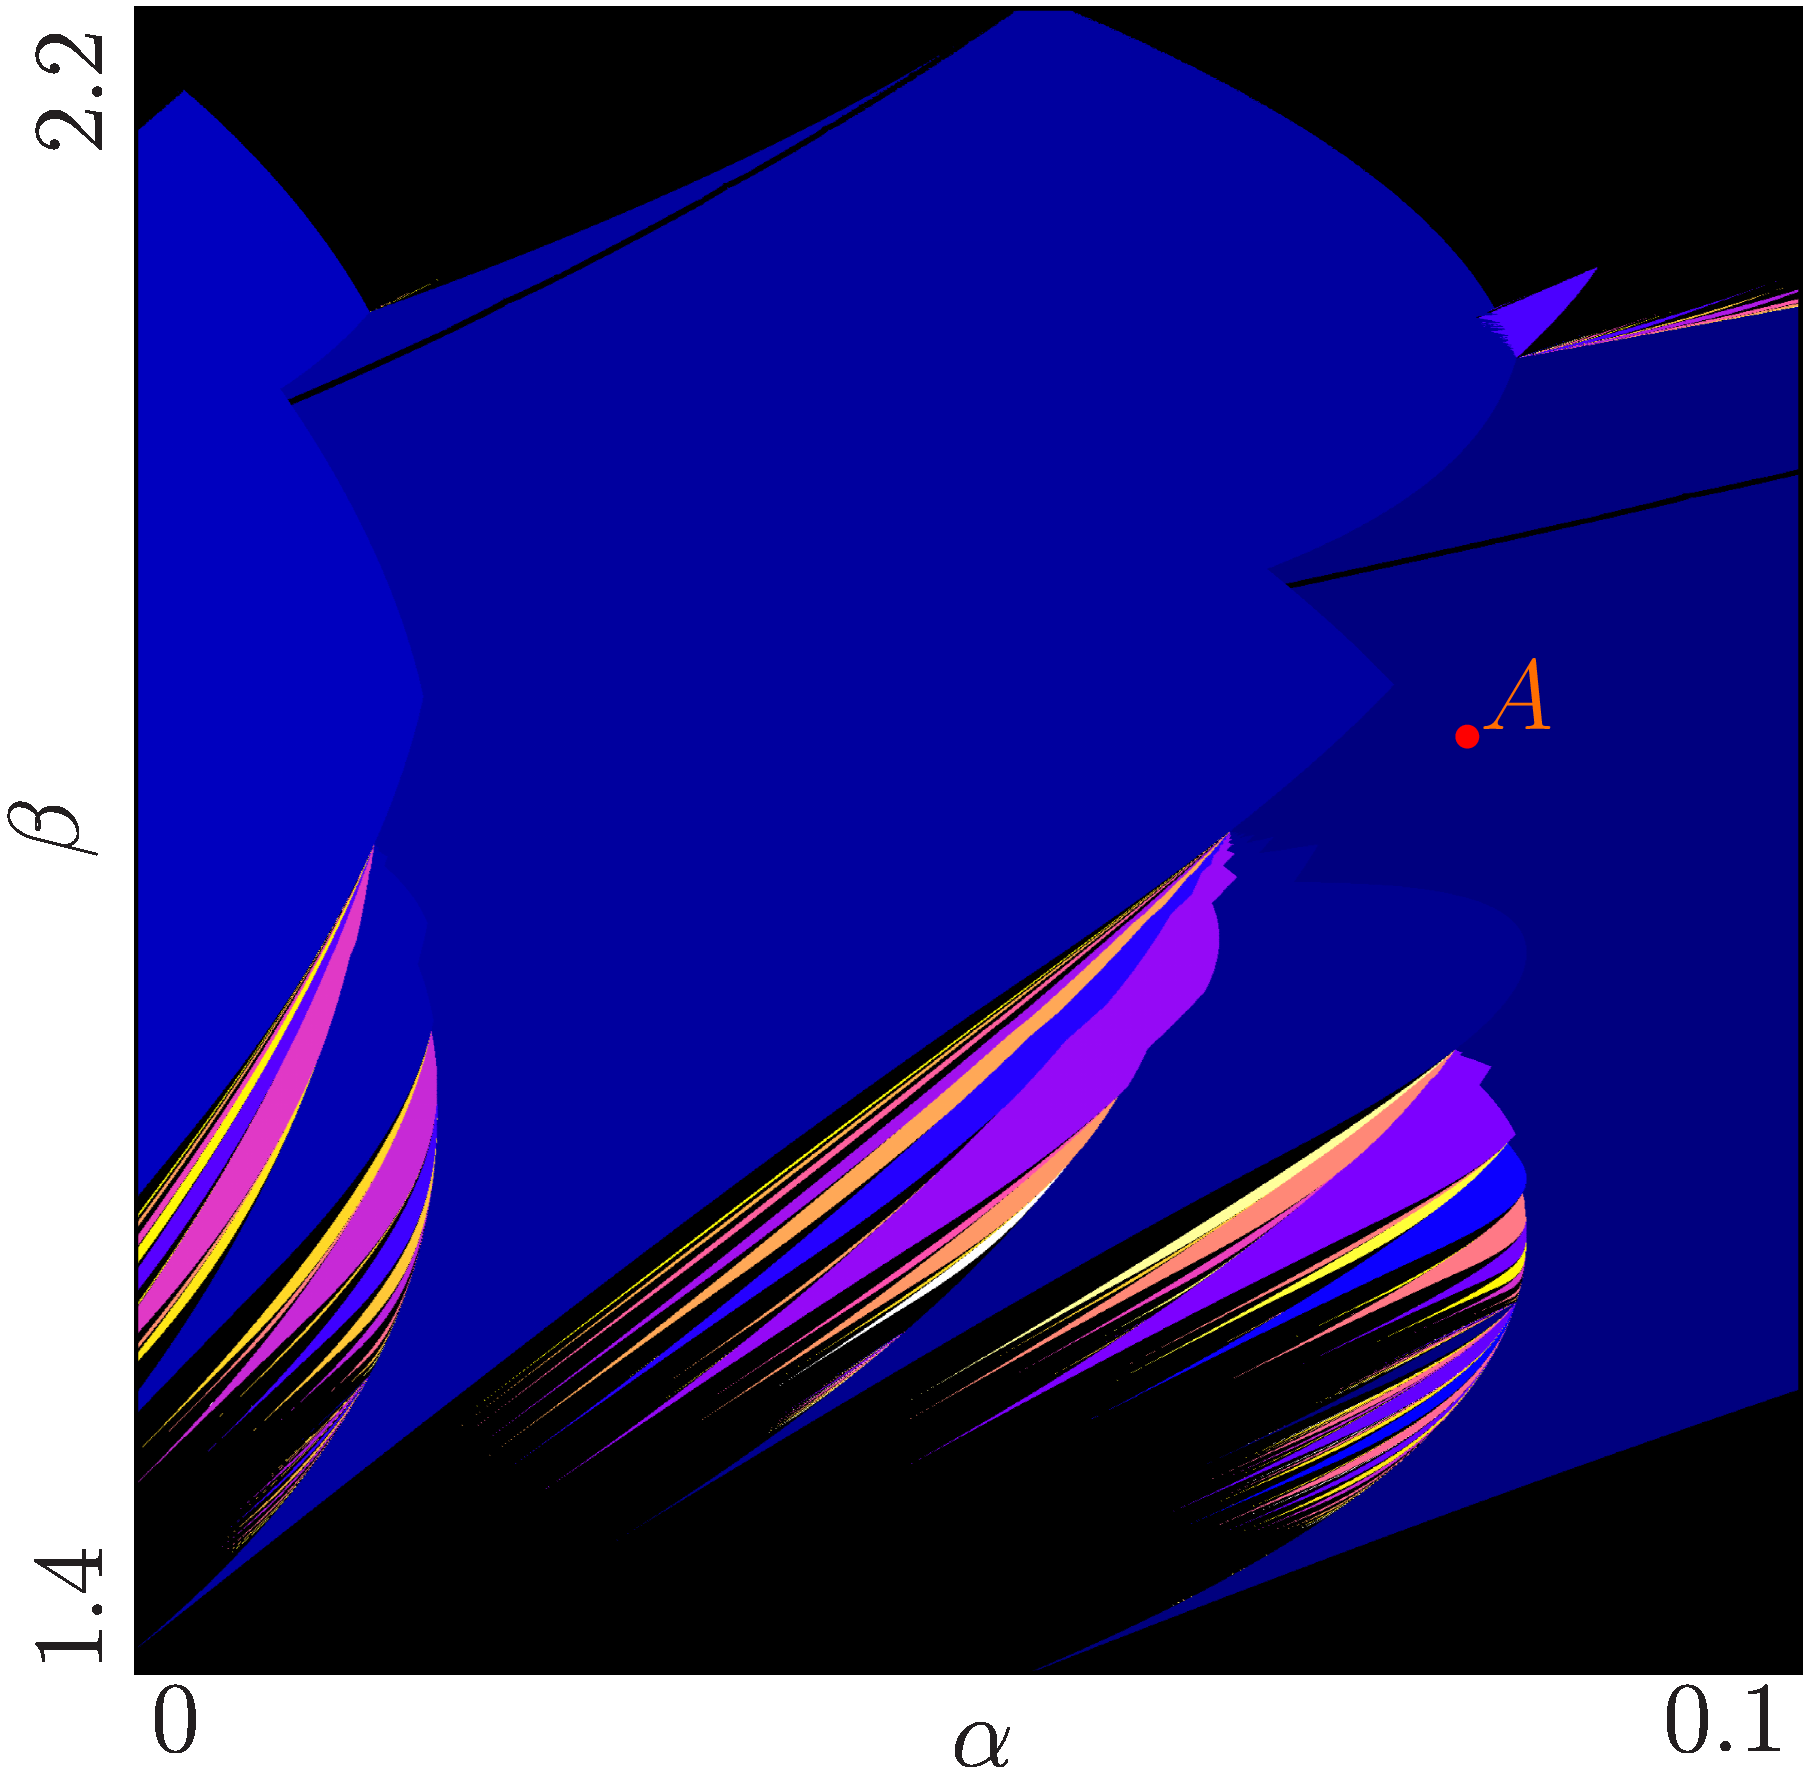
\includegraphics[width=.7 \textwidth]{../Figures/A/A.2a/result.png}
		\label{fig:app.model.quad.first}
	} \\
	\subfloat[Cobweb diagram]{
		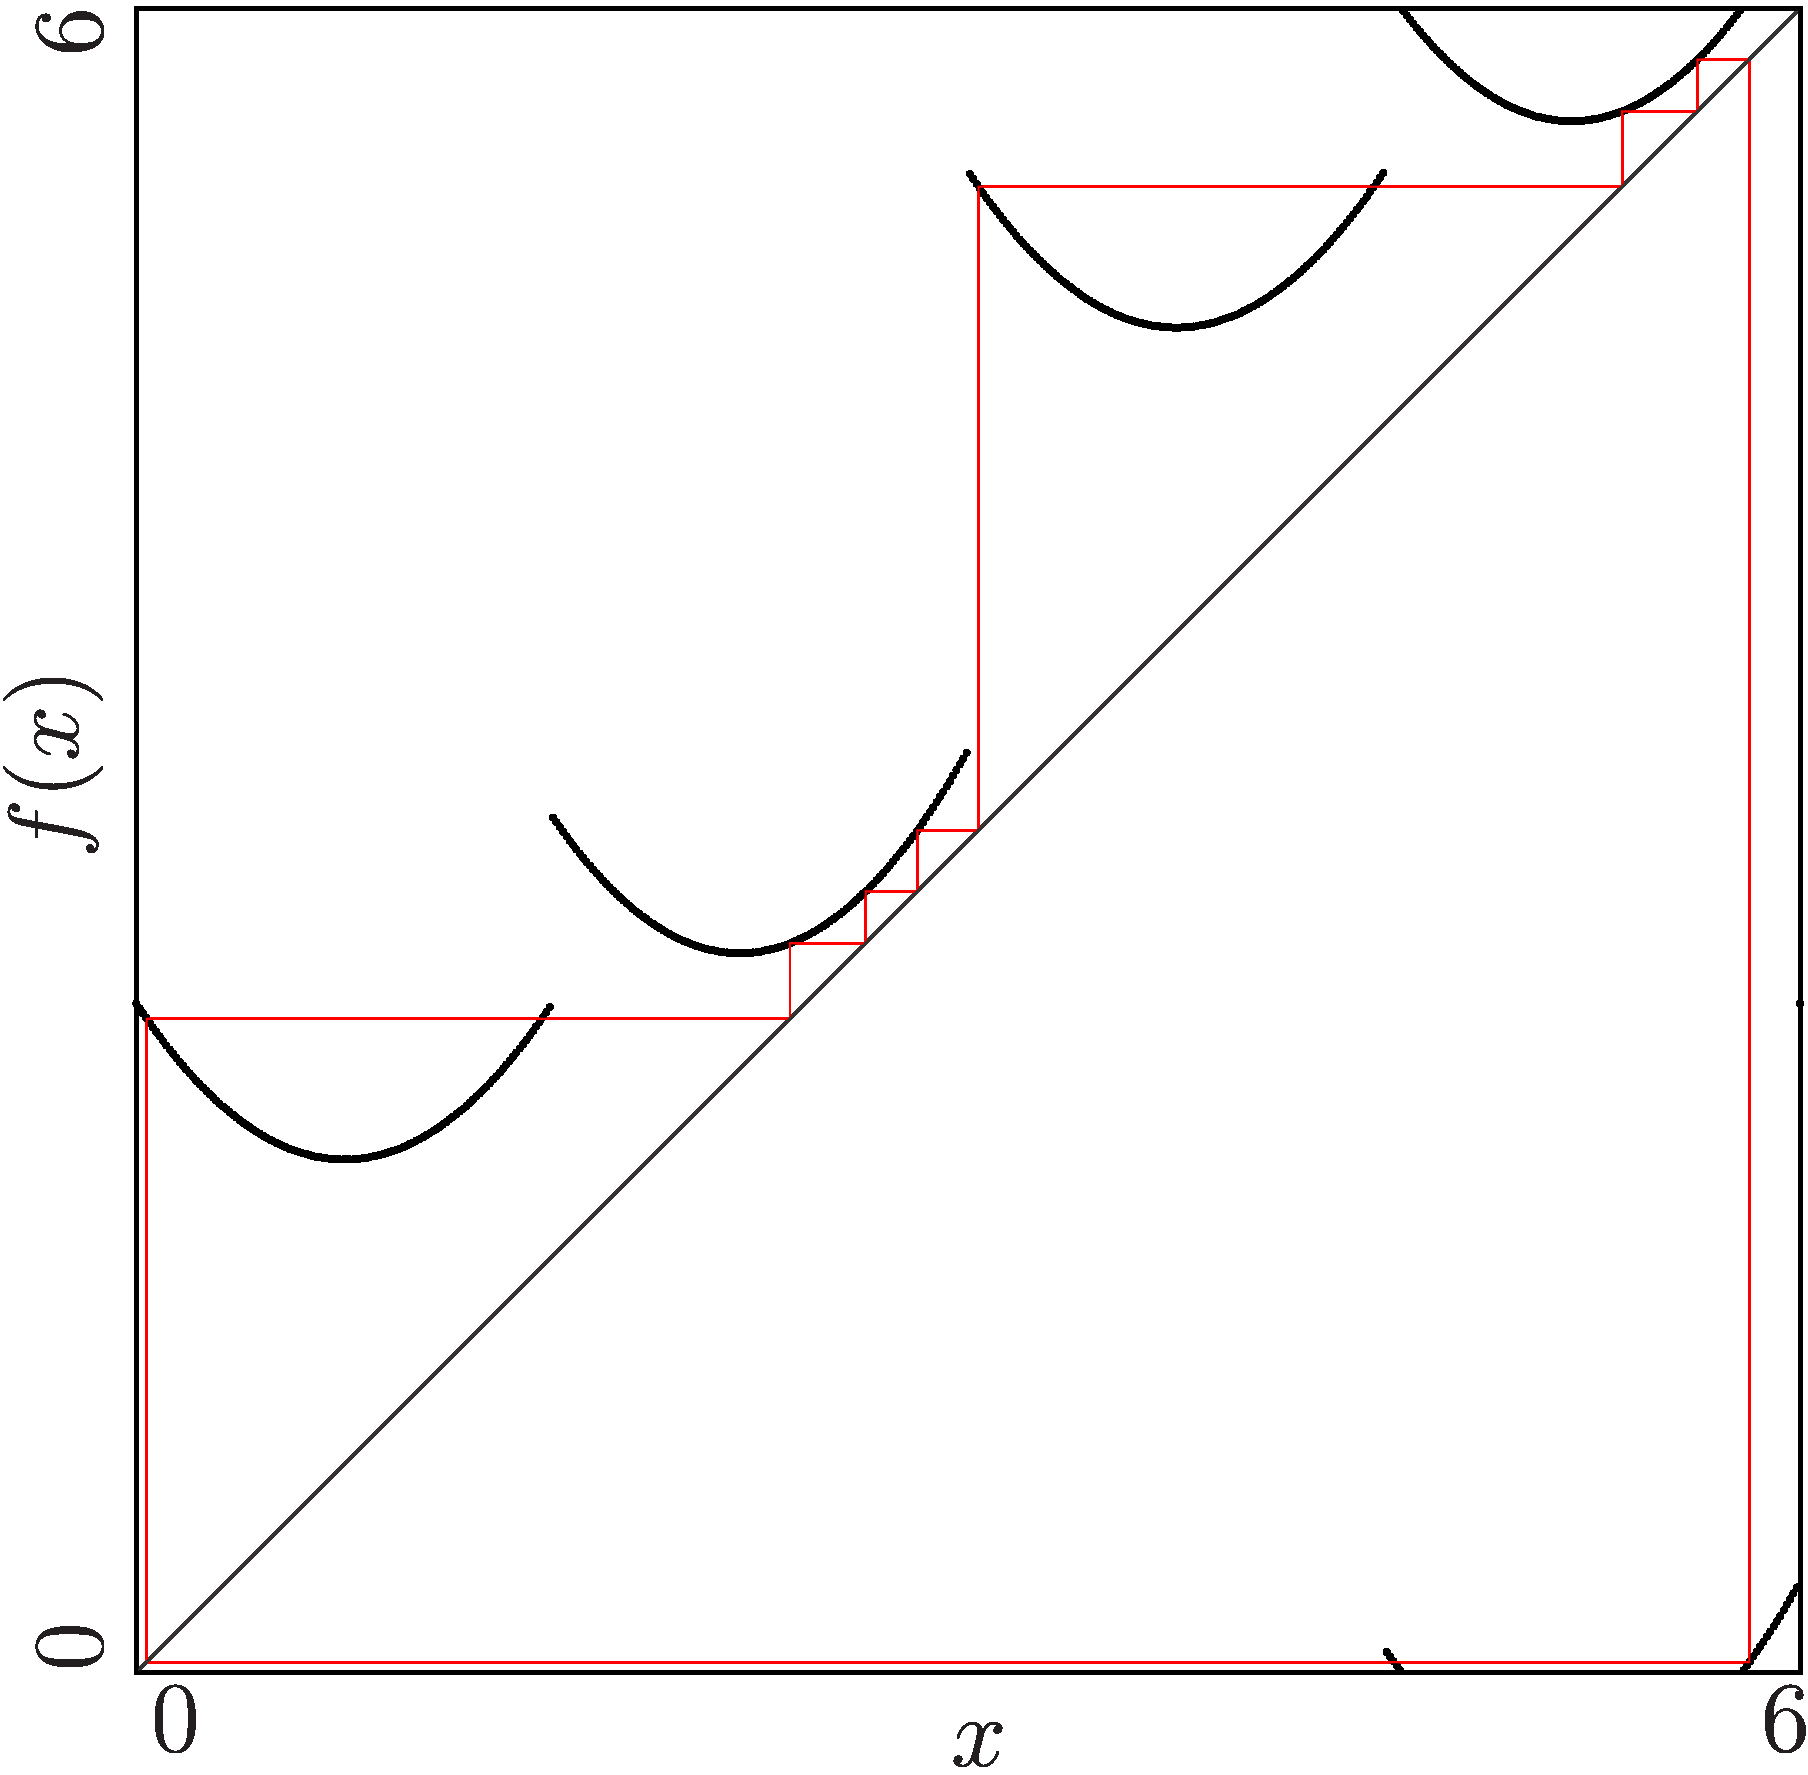
\includegraphics[width=.5 \textwidth]{../Figures/A/A.2b/result.png}
		\label{fig:app.model.quad.first.cob}
	}
	\caption[2D scan of the periods associated with parameter regions in the piecewise-quadratic model with composite parameters and an exemplary cobweb diagram]{
		2D scan of the periods associated with parameter regions in the piecewise-quadratic model with composite parameters and an exemplary cobweb diagram.
		The parameters $a_L = 1, b_L = 0,$ and $c_R = 2.6$ are fixed.
		The parameters $a_R = 1 + \alpha$ and $b_R = 2 \cdot \alpha$ depend on the varied parameter $\alpha$.
		And the parameters $\alpha$ and $\beta$ are different in each diagram.
		(a) shows the 2D scan with the parameters $\alpha$ and $\beta$ being varied in the ranges $[0, 0.1]$ and $[1.4, 2.2]$,
		(b) shows the exemplary cobweb diagram of the cycle at the point $A$ marked in (a) where $\alpha = 0.08$ and $\beta = 1.85$.
	}
\end{figure}

\clearpage
\subsection{Second Choice of Composite Parameters}

The parameters $a_R = 1 + 2 \cdot \alpha$ and $b_R = \alpha$ are chosen.
This is similar to the first choice of composite parameters, but this time $\alpha$ influences the parameter $a_R$ more and $b_R$ less.
The other varied parameter is still $\beta = c_L$.

\Cref{fig:app.model.quad.second} shows a 2D scan of the periods of cycles associated with parameter regions in the piecewise-quadratic model with the parameter choices above.
Again, we can see wing-shaped parameter regions.
The big parameter regions are now oriented horizontally, but they still seem to form a \gls{pi} cascade.
Also, there are smaller parameter regions between the bigger ones that seem to form \gls{pa} structures.

Something, we did not see before that is present here are hybrid parameter regions.
\Cref{fig:app.model.quad.second.cob} shows a cobweb diagram at the parameter values marked with the point $A$ in \Cref{fig:app.model.quad.second}.
It shows the twin cycles $\Cycle{A^4\B\C^2\D}$ and $\Cycle{A^2\B\C^4\D}$ coexisting.

\begin{figure}
	\centering
	\subfloat[2D scan]{
		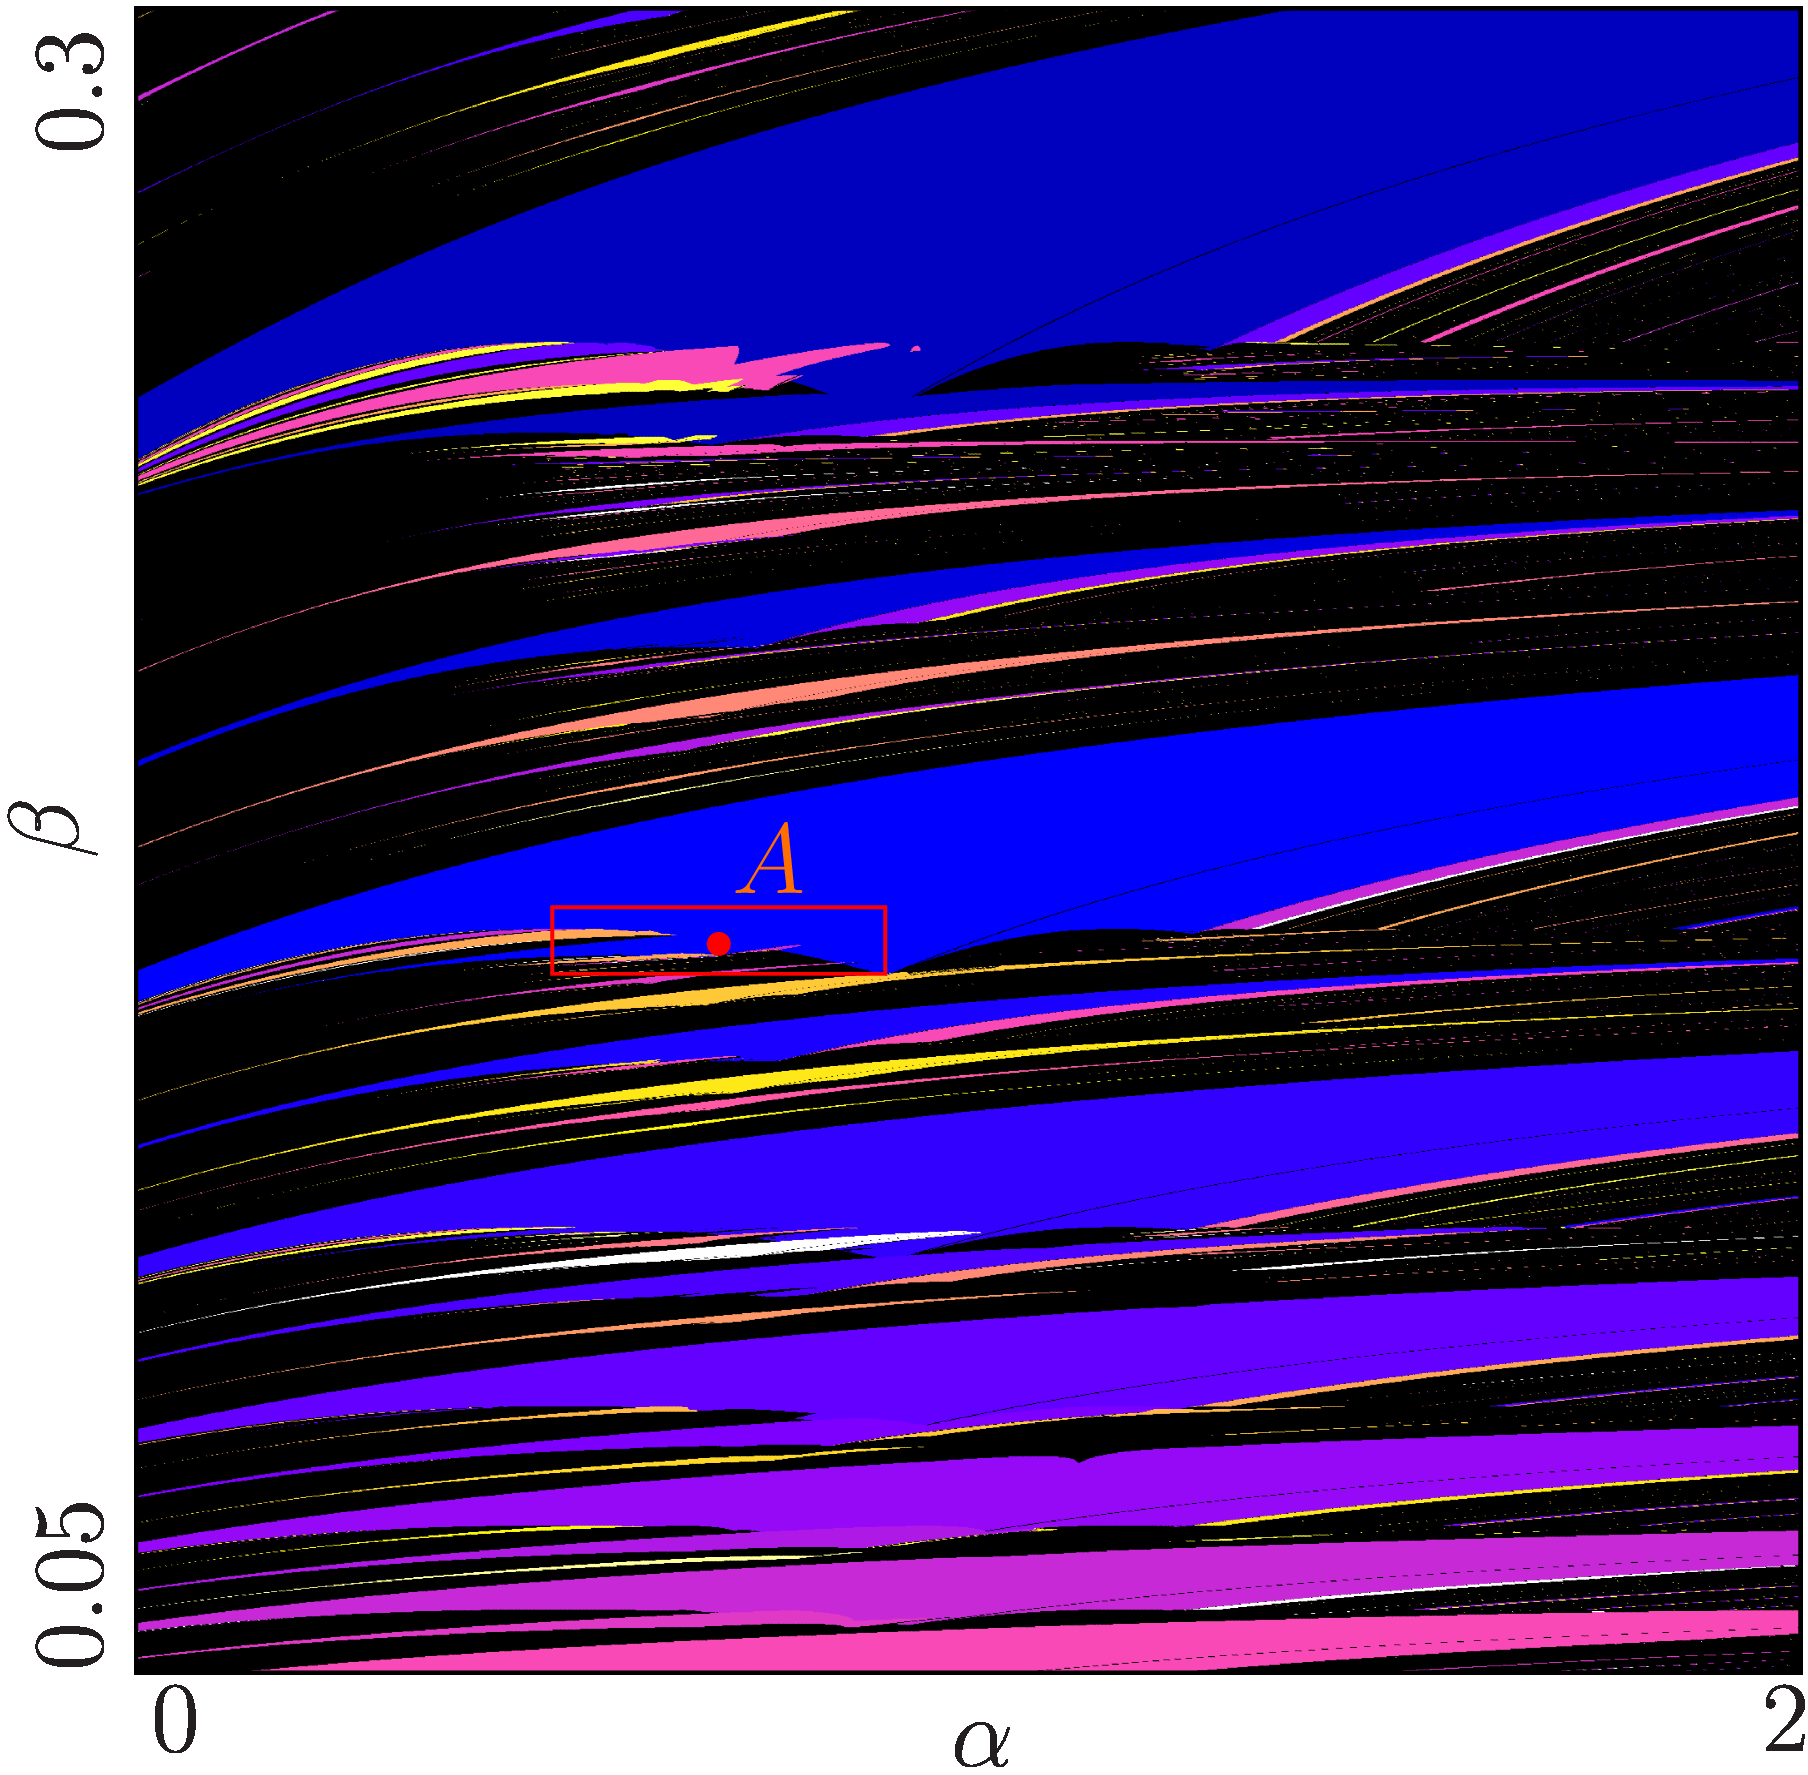
\includegraphics[width=.7 \textwidth]{../Figures/A/A.3a/result.png}
		\label{fig:app.model.quad.second}
	} \\
	\subfloat[Cobweb diagram]{
		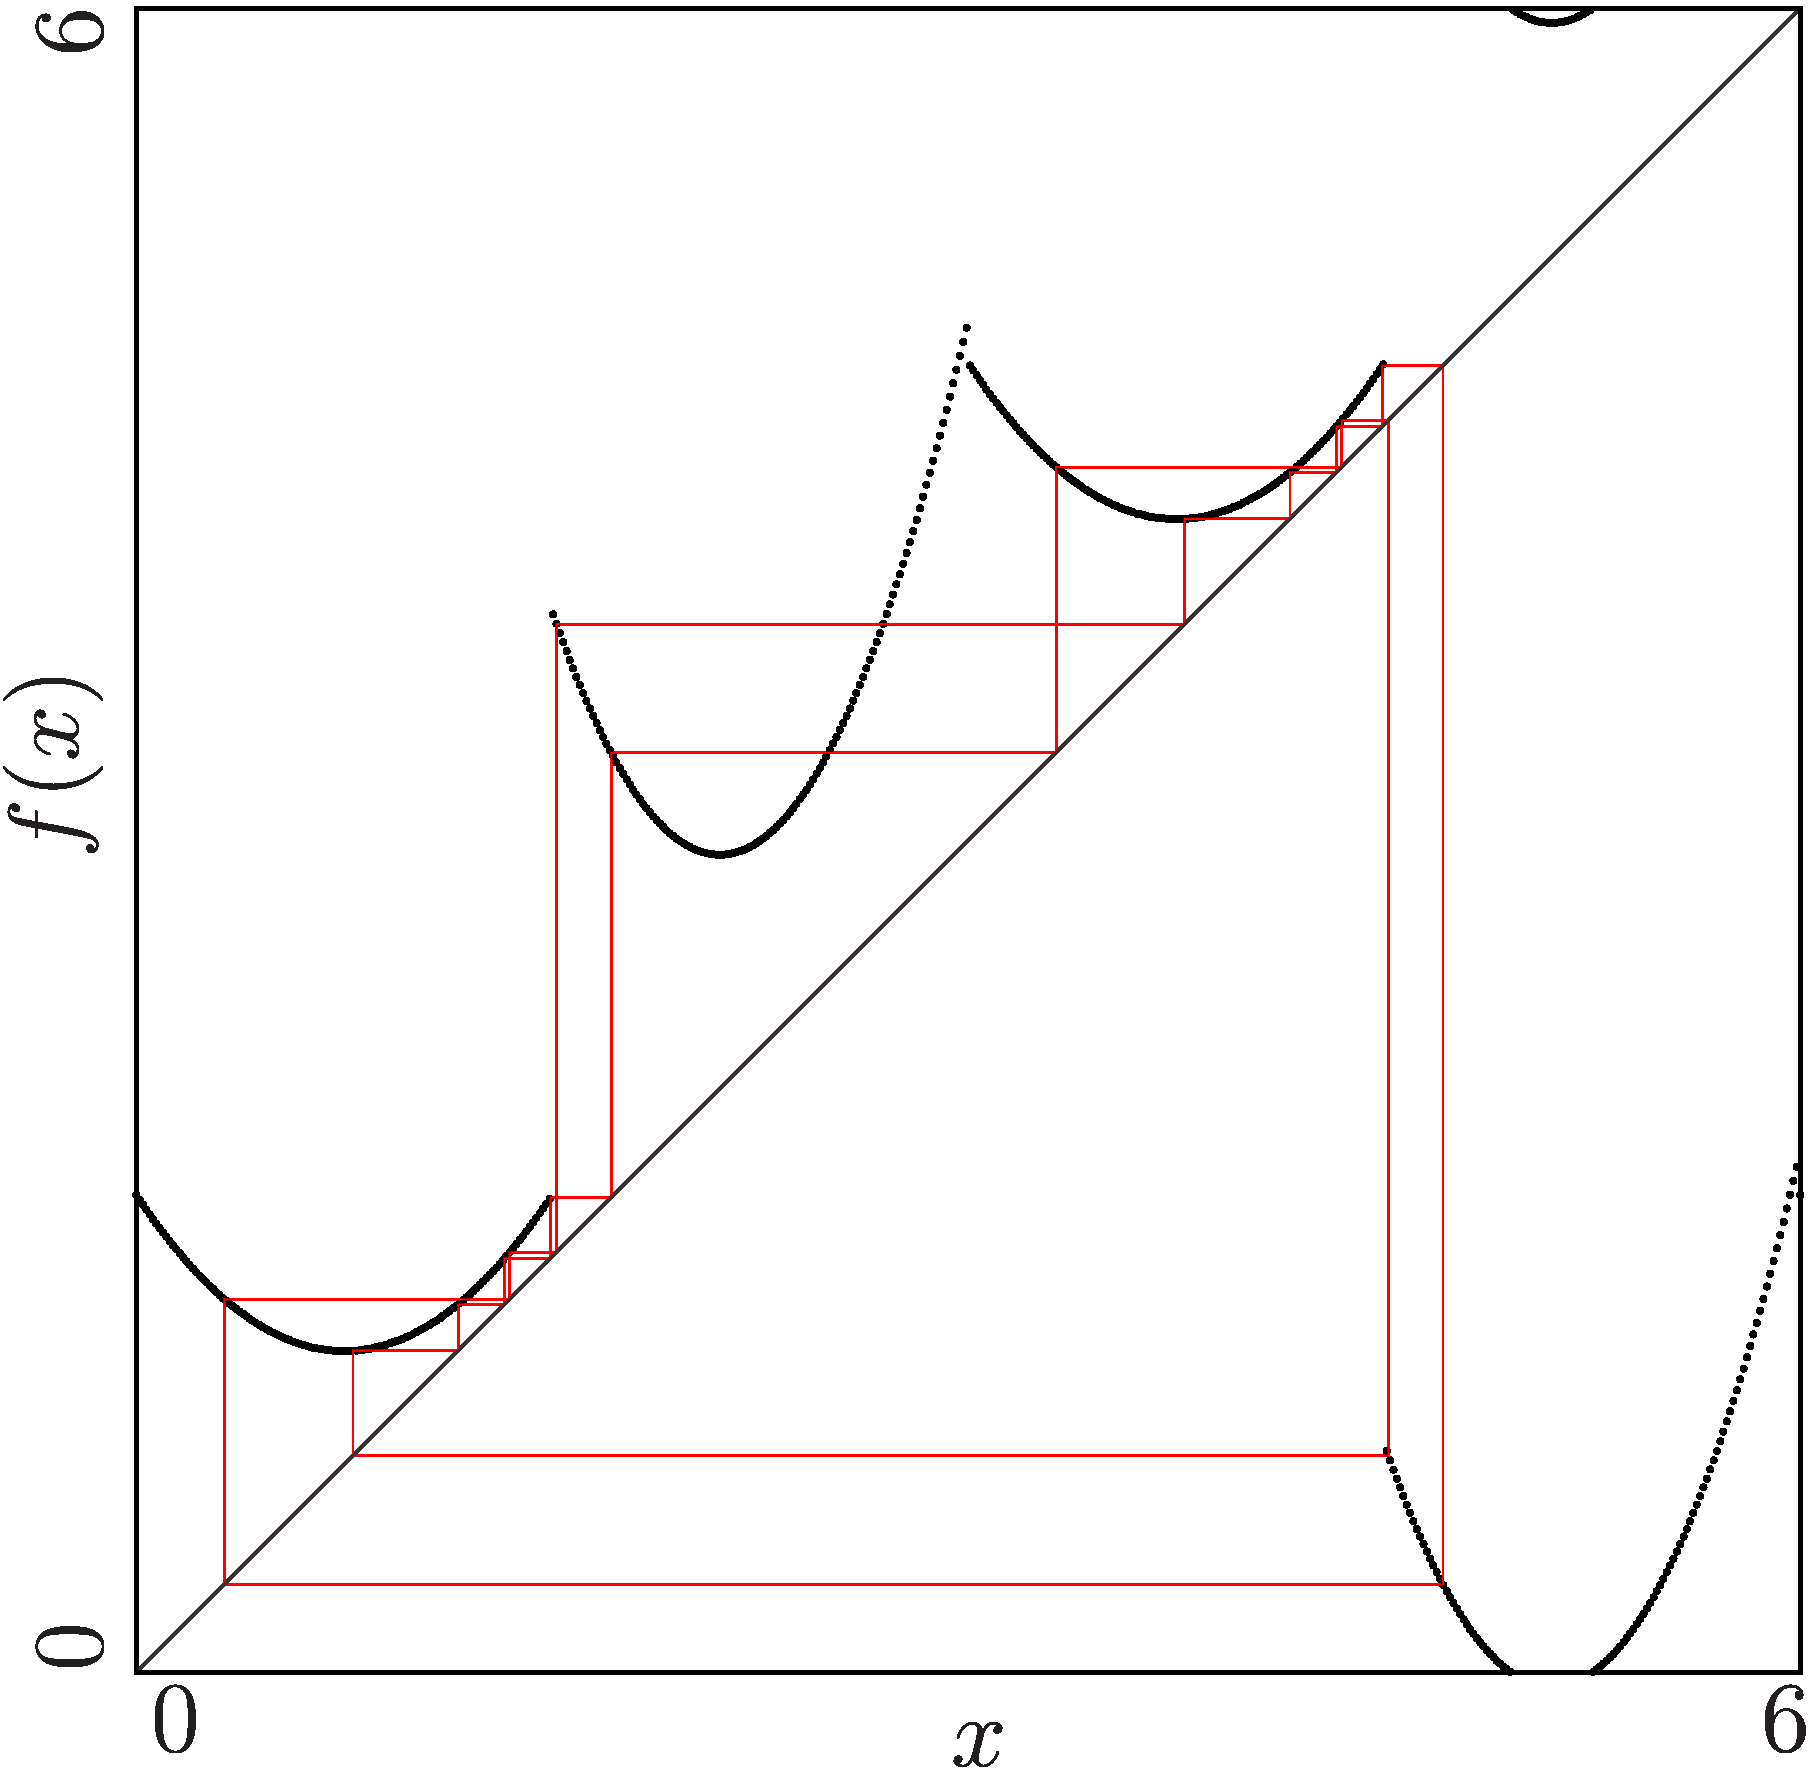
\includegraphics[width=.5 \textwidth]{../Figures/A/A.3b/result.png}
		\label{fig:app.model.quad.second.cob}
	}
	\caption[2D scan of the periods associated with parameter regions in the piecewise-quadratic model with composite parameters and an exemplary cobweb diagram]{
		2D scan of the periods associated with parameter regions in the piecewise-quadratic model with composite parameters and an exemplary cobweb diagram.
		The parameters $a_L = 1, b_L = 0,$ and $c_R = 2.6$ are fixed.
		The parameters $a_R = 1 + \alpha$ and $b_R = 2 \cdot \alpha$ depend on the varied parameter $\alpha$.
		And the parameters $\alpha$ and $\beta$ are different in each diagram.
		(a) shows the 2D scan with the parameters $\alpha$ and $\beta$ being varied in the ranges $[0, 0.1]$ and $[1.4, 2.2]$,
		(b) shows the exemplary cobweb diagram of the cycle at the point $A$ marked in (a) where $\alpha = 0.08$ and $\beta = 1.85$.
	}
\end{figure}

\clearpage
\subsection{Mirrored Configuration Based on the Second Choice of Composite Parameters}

The marked parameter range in \Cref{fig:app.model.quad.second} is interesting, because here two wing-shaped parameter regions overlap.
The lower parameter region is a hybrid parameter region that is associated with the twin cycles $\Cycle{A^4\B\C^2\D}$ and $\Cycle{A^2\B\C^4\D}$ while the upper parameter region is associated with the cycle $\Cycle{\A^4\B\C^4\D}$.

\begin{figure}
	\centering
	\subfloat[]{
		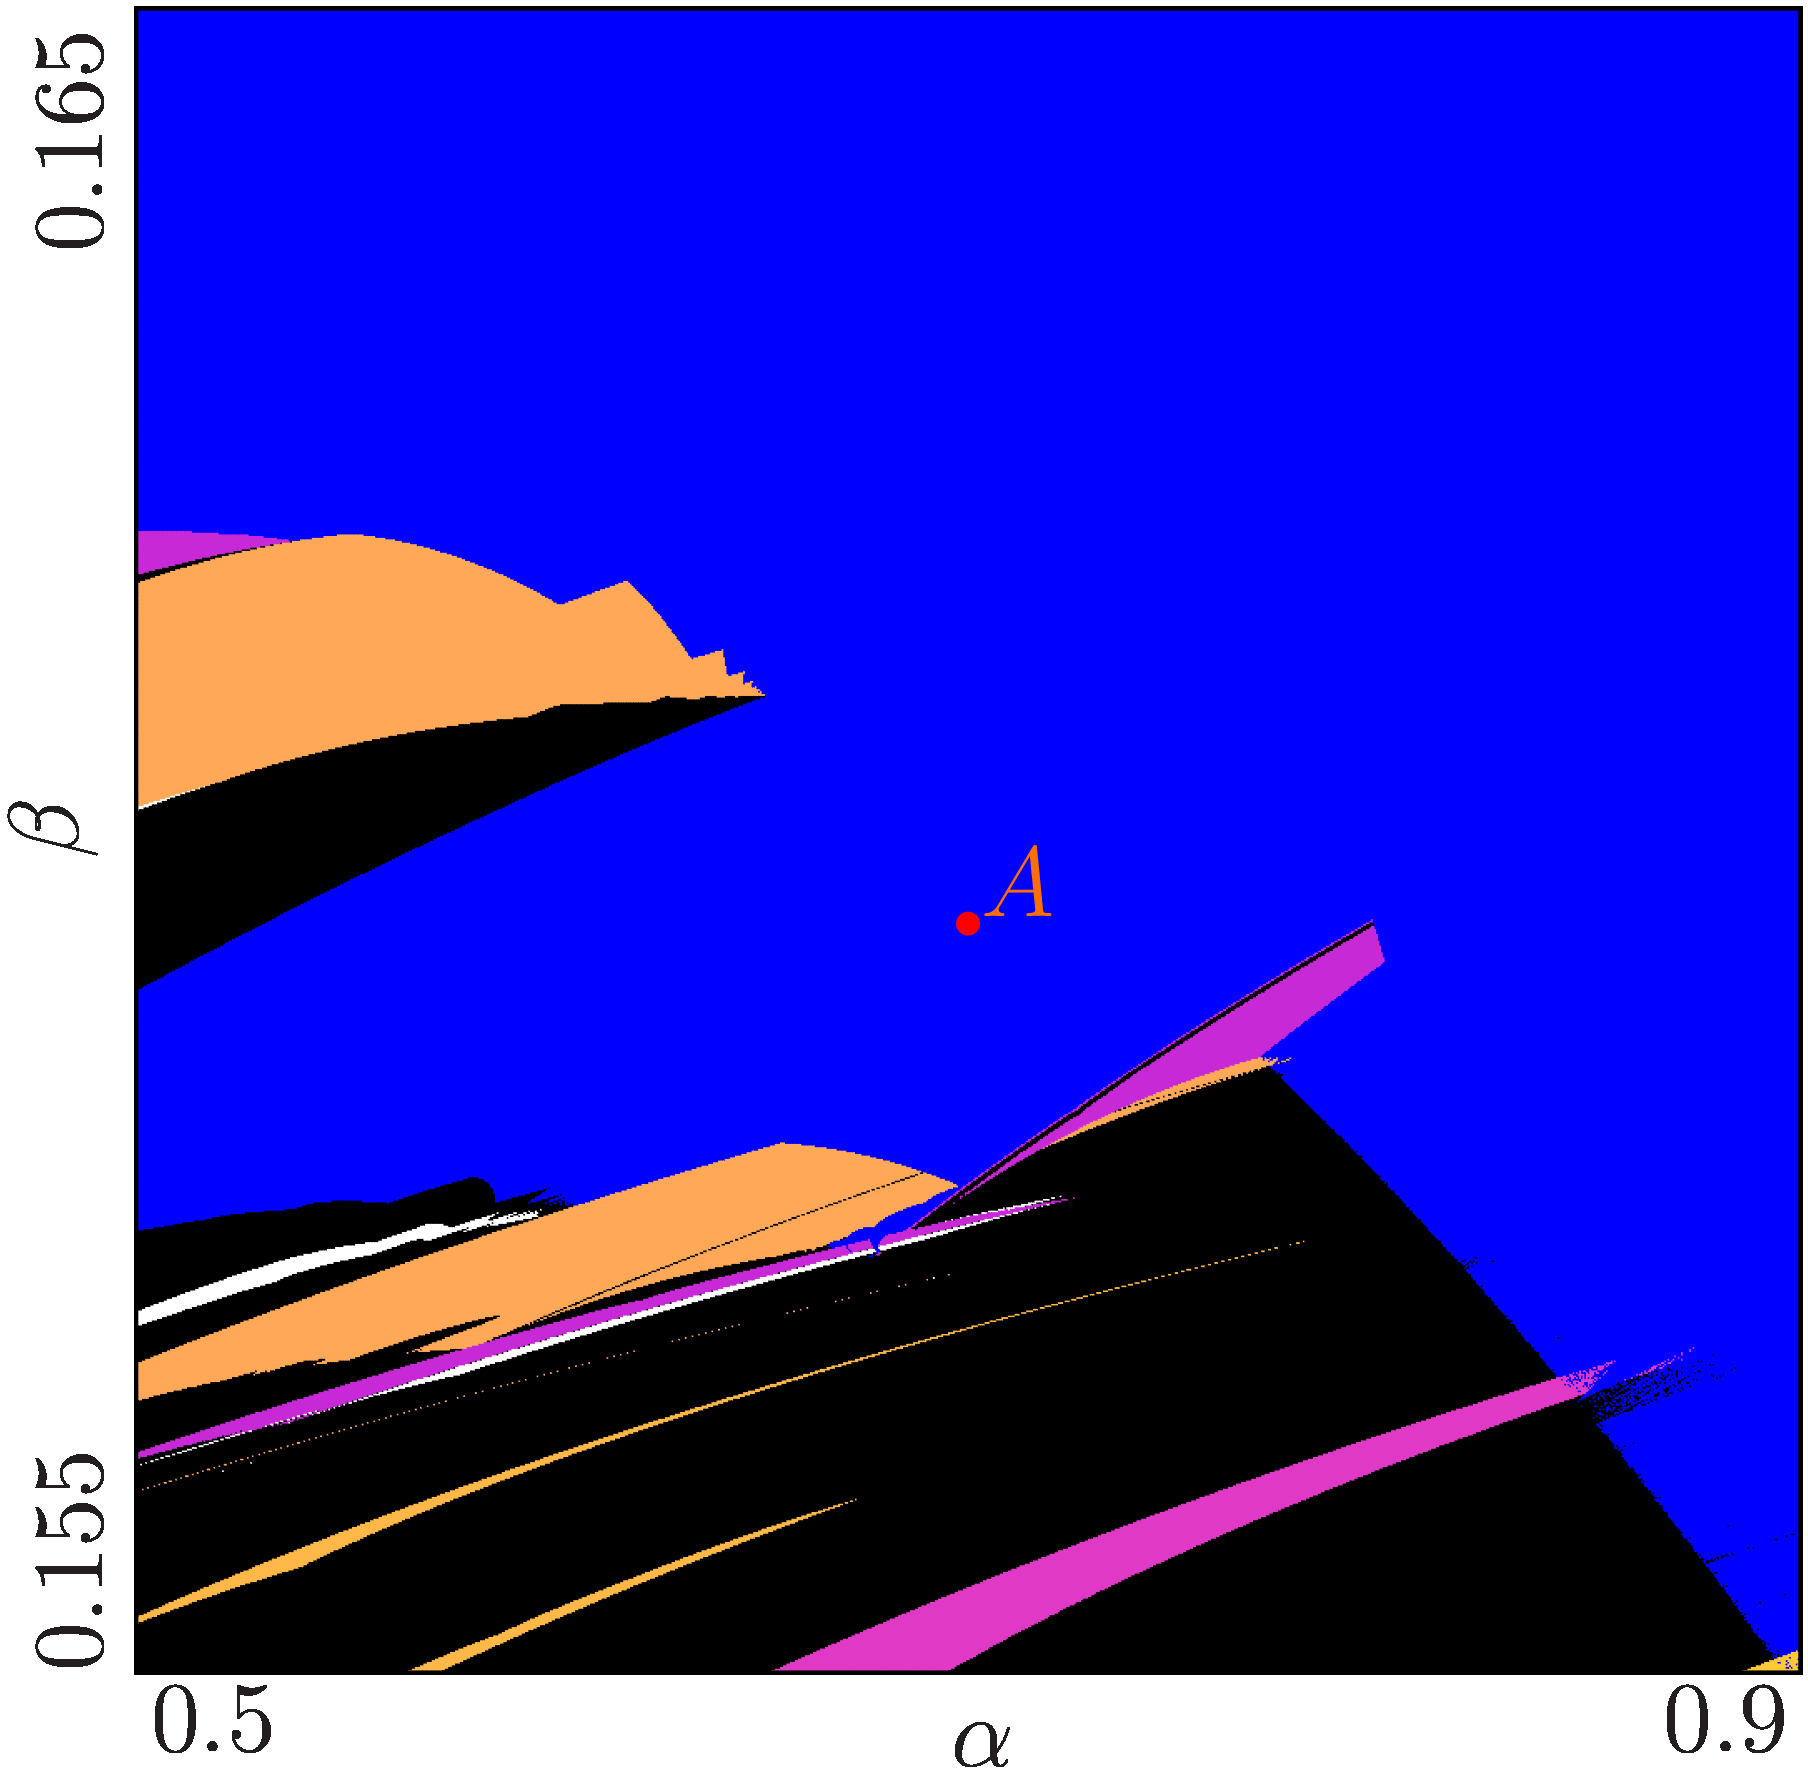
\includegraphics[width=.4 \textwidth]{../Figures/A/A.4a/result.png}
		\label{fig:app.model.quad.second.zoomed}
	} \\
	\subfloat[]{
		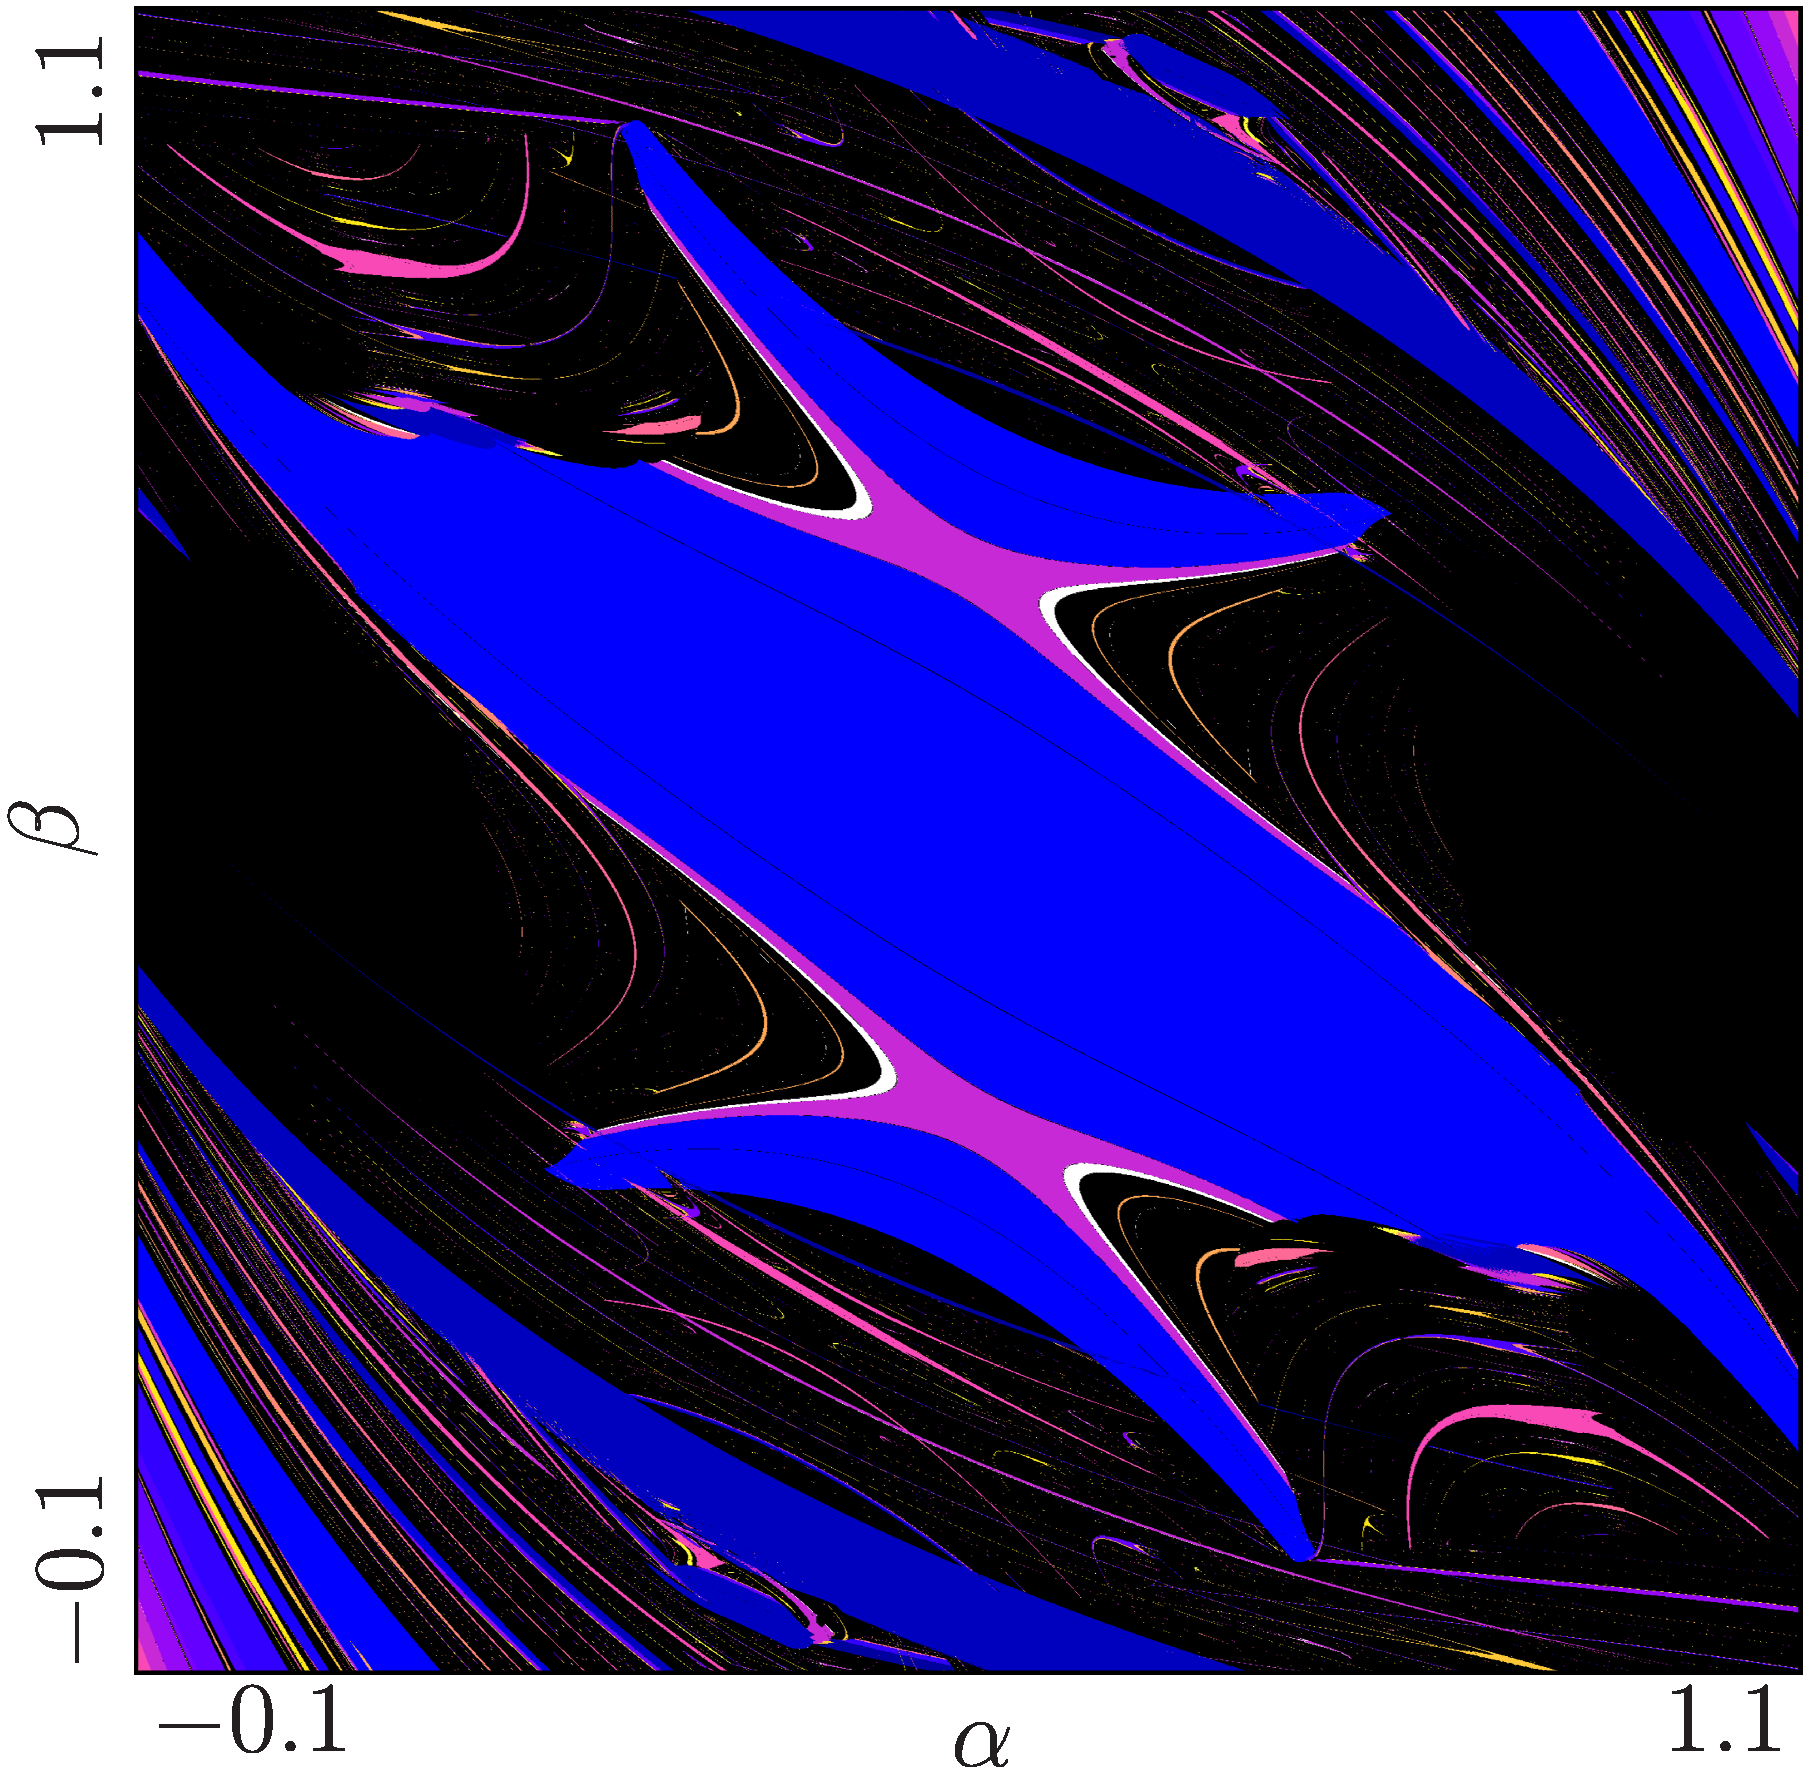
\includegraphics[width=.7 \textwidth]{../Figures/A/A.4b/result.png}
		\label{fig:app.model.quad.mirrored}
	}
	\caption[2D scan of the periods associated with parameter regions in the mirrored piecewise-quadratic model]{
		2D scan of the periods associated with parameter regions in the mirrored piecewise-quadratic model
		(a) show a magnified version of \Cref{fig:app.model.quad.second} with parameters $\alpha$ and $\beta$ varied in the ranges $[0.5, 0.9]$ and $[0.155, 0.165]$ which is marked with a red rectangle in \Cref{fig:app.model.quad.second}.
		(b) shows the 2D scan of another model that has the same parameters as the model above at the point marked with $A$ in (a) at $\alpha = 0$ and $\beta = 0$ but has the configuration where the parameters of $g_L$ and $g_R$ are swapped for $\alpha = 1$ and $\beta = 1$ as explained above.
	}
\end{figure}

Now the parameters $\alpha$ and $\beta$ are chosen very differently.
The parameters are chosen in such a way that for $\alpha = \beta = 0$, the parameter values are precisely the same as the parameter values that are marked with the point $A$ in \Cref{fig:app.model.quad.second.zoomed}.
And for $\alpha = \beta = 1$, the parameter values are precisely the same but $a_L$ is swapped with $a_R$, $b_L$ with $b_R$, and $c_L$ with $c_R$.
The goal is to force the model to form a chain from a parameter region associated with two coexisting twin cycles $\Cycle{A^4\B\C^2\D}$ and $\Cycle{A^2\B\C^4\D}$ to a parameter regions associated with two twin cycles $\Cycle{A\B^4\C\D^2}$ and $\Cycle{A\B^2\C\D^4}$.
Ideally with ``type A'' parameter regions and one point after the other moving from the branches $\A$ and $\C$ to $\B$ and $\D$.

$\alpha$ should only influence the parameters $a_L, b_L, a_R,$ and $b_r$, while $\beta$ should only influence $c_L$ and $c_R$.
With these constraints, we arrive at the following values for $a_L, b_L, c_L, a_R, b_R,$ and $c_R$ in dependence of $\alpha$ and $\beta$.

\begin{subequations}
	\begin{align}
		a_L & = 1 + \frac{3}{2} \cdot \alpha           \\
		b_L & = \frac{3}{4} \cdot \alpha               \\
		c_L & = 1.1605 + 0.3395 \cdot \beta            \\
		a_R & = 2.5 - \frac{3}{2} \cdot \alpha         \\
		b_R & = \frac{3}{4} - \frac{3}{4} \cdot \alpha \\
		c_R & = 3 - 0.3395 \cdot \beta
	\end{align}
\end{subequations}

\Cref{fig:app.model.quad.mirrored} shows a 2D scan of the periods of the cycles associated with the parameter regions in the piecewise-quadratic model with the parameter values chosen above.
We see that it is symmetric, which we would expect, since we chose the parameters $\alpha$ and $\beta$ were chosen with that goal in mind.
Unfortunately there are no chains with this choice of parameters either.
